\documentclass[9pt,twocolumn,twoside]{osajnl}
%% Please use 11pt if submitting to AOP
% \documentclass[11pt,twocolumn,twoside]{osajnl}
\usepackage{graphicx}% Include figure files
\usepackage{dcolumn}% Align table columns on decimal point
\usepackage{bm}% bold math
\usepackage{natbib}
\usepackage{physics}

\journal{optica} % Choose journal (ao, aop, josaa, josab, ol, optica, pr)

% See template introduction for guidance on setting shortarticle option
\setboolean{shortarticle}{true}
% true = letter / tutorial
% false = research / review article
% (depending on journal).

\title{Legacy \LaTeX\ template for preparing an article for submission to OSA journals \emph{Applied Optics}, \emph{Advances in Optics and Photonics}, JOSA A, JOSA B, \emph{Optics Letters}, \emph{Optica}, and \emph{Photonics Research}}

\author[1,2,3]{Author One}
\author[2,*]{Author Two}
\author[1]{Author Three}

\affil[1]{Publications Department, The Optical Society (OSA), 2010 Massachusetts Avenue NW, Washington D.C., 20036}
\affil[2]{School of Science, University of Technology, 2000 J St. NW, Washington DC, 20036}
\affil[3]{School of Optics, University of Technology, 2000 J St. NW, Washington DC, 20036}

\affil[*]{Corresponding author: email@my-email.com}

%% To be edited by editor
% \dates{Compiled \today}

%\ociscodes{(140.3490) Lasers, distributed feedback; (060.2420) Fibers, polarization-maintaining;(060.3735) Fiber Bragg gratings.}

%% To be edited by editor
% \doi{\url{http://dx.doi.org/10.1364/XX.XX.XXXXXX}}

\begin{abstract}
This legacy template can be used to prepare a research article for submission to OSA’s journals \emph{Applied Optics}, \emph{Advances in Optics and Photonics}, JOSA A, JOSA B, \emph{Optics Letters}, and \emph{Optica}. \emph{Optics Letters} authors and authors of \emph{Optica} letters and memoranda may use this template for a precise length estimate. Use the shortarticle/true option for \emph{Optics Letters} and short \emph{Optica} articles. 
\end{abstract}

\setboolean{displaycopyright}{true}

\begin{document}

\maketitle

\section{Introduction}
This legacy template is designed to assist with creating an article to submit to \emph{Applied Optics}, \emph{Advances in Optics and Photonics}, JOSA A, JOSA B, \emph{Optics Letters} or \emph{Optica}. See the OSA's \href{http://www.opticsinfobase.org/submit/style/}{Style Guide} and \href{http://www.opticsinfobase.org/submit/templates/}{Manuscript Templates} pages for more details. Please select the appropriate journal abbreviation (ao, aop, josaa, josab, ol, optica) in the document preamble.

Use the shortarticle/false option for \emph{Applied Optics}, JOSA A, and JOSA B. Use the shortarticle/true option for \emph{Optics Letters}. For \emph{Advances in Optics and Photonics}, use the shortarticle/false option for Review Articles, and the shortarticle/true option for Tutorials.

If you have a question while using this template on {Overleaf}, please use the help menu (``?'') on the top bar to search for help or ask us a question using our \href{https://www.overleaf.com/contact}{contact form}.

\section{Examples of Article Components}
\label{sec:examples}

The sections below show examples of different article components.

\section{Figures and Tables}

It is not necessary to place figures and tables at the back of the manuscript. Figures and tables should be sized as they are to appear in the final article. Do not include a separate list of figure captions and table titles.

Figures and Tables should be labelled and referenced in the standard way using the \verb|\label{}| and \verb|\ref{}| commands.



\begin{figure}[htbp]
\centering
\fbox{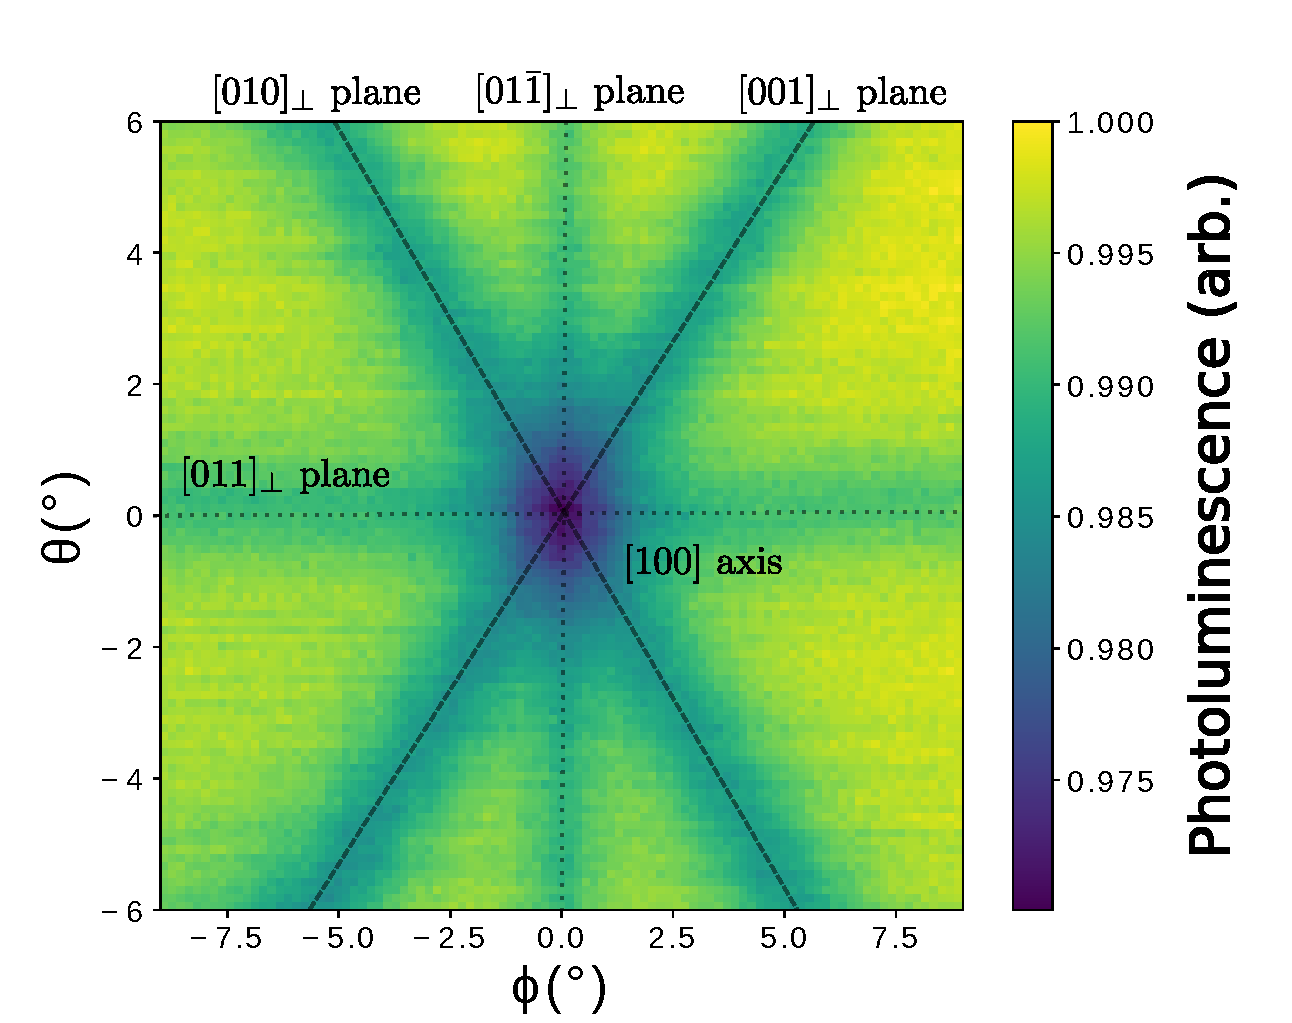
\includegraphics[width=\linewidth]{Carte_annotation}}
\caption{NV$^-$ photoluminescence as a function of a scanning magnetic field around the [100] crystalline directions with a fixed amplitude $|B|=115G$. The planes orthogonal to the [010],[001],[011], and [01$\bar 1$] directions are indicated in dashed lines.}
\label{map}
\end{figure}

\begin{figure}[htbp]
\centering
\fbox{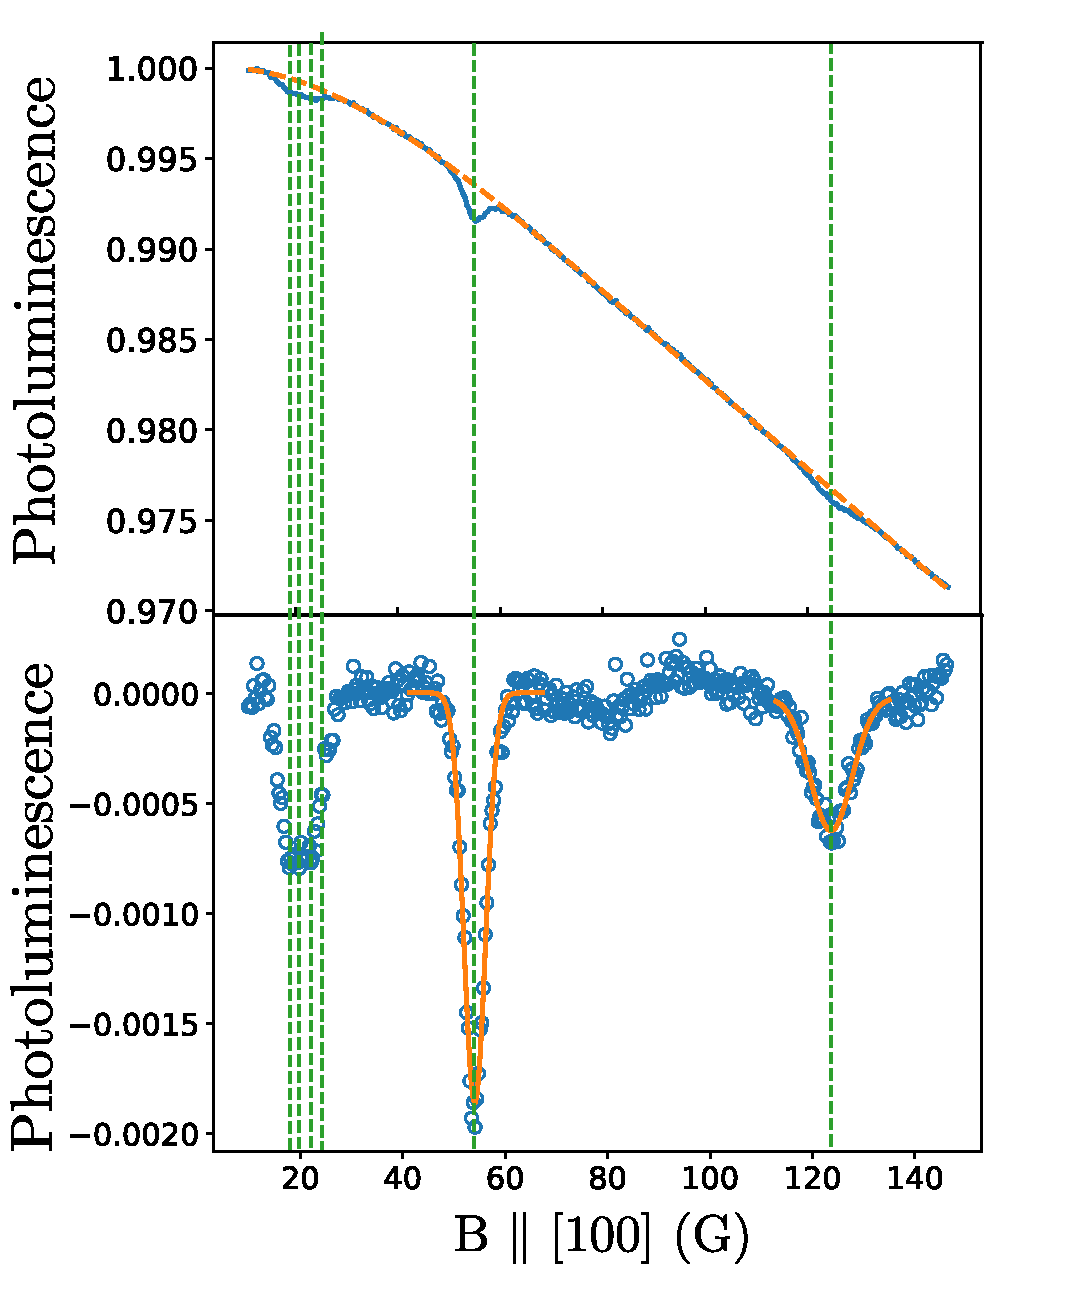
\includegraphics[width=\linewidth]{Scans_fig4}}
\caption{Optical detection of cross-relaxations. \textbf{Top} NV$^-$ photoluminescence while scanning the magnetic field along the [100] crystalline direction (plain line) and polynomial fit to the fourth order (dashed line). \textbf{Bottom} Subtraction of the previous signal by the polynomial fit (circles), simulated CR magnetic field amplitude (dashed,vertical) and gaussian fits for the second and third dips (plain line)}
\label{scan}
\end{figure}

\begin{figure}[htbp]
\centering
\fbox{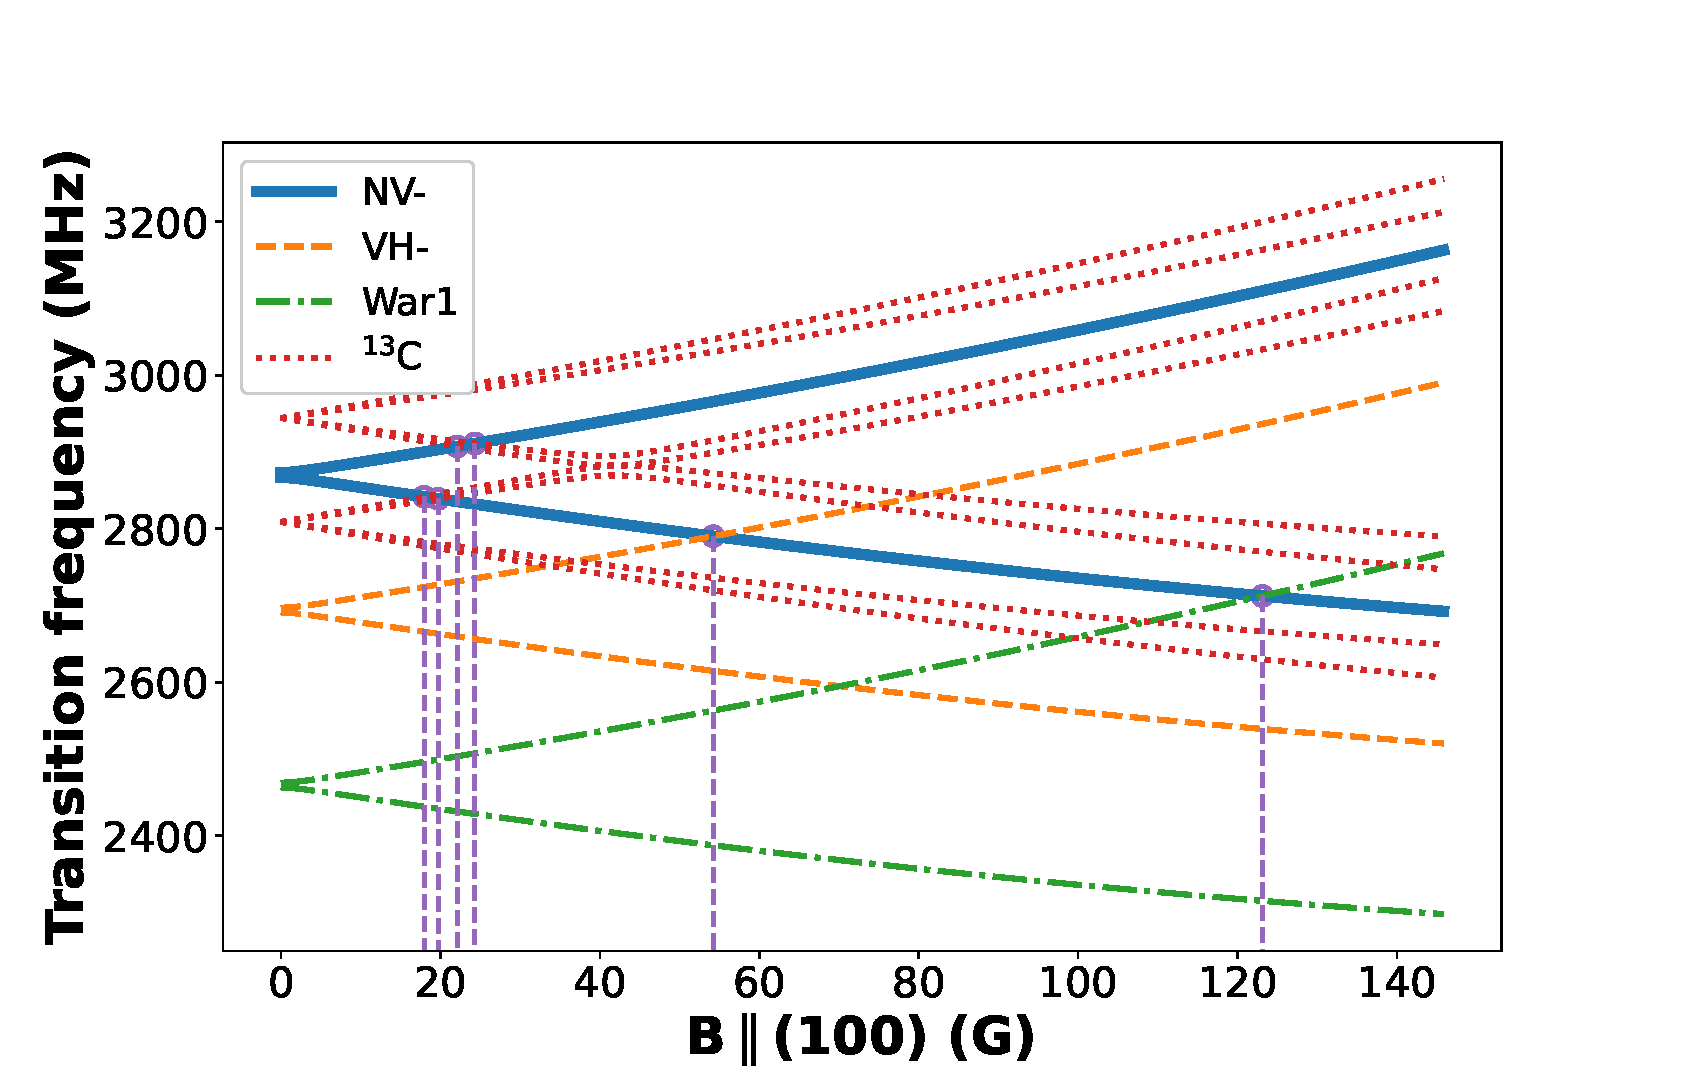
\includegraphics[width=\linewidth]{Theorie_CR}}
\caption{Simulated energy levels as a function of a magnetic field aligned along the [100] axis for the various spins considered. NV centers are in plain lines, VH$^-$ are in dashed line, WAR1 in dashdotted line and $^{13}$C-NV pair in dotted line. The amplitudes of the magnetic field where the energy level of the NV center crosses the one of another species are represented by vertical dashed lines}
\label{energy-levels}
\end{figure}

\subsection{Sample Table}

Table \ref{tab:shape-functions} shows an example table.

\begin{table}[htbp]
\centering
\caption{\bf Zero-field splitting parameter $D_z$ for the different spin-1 species}
\begin{tabular}{ccc}
\hline
$D_z$ estimation (MHz) & Cruddace's work\citep{cruddace2007magnetic} & Our work \\
\hline
NV$^-$ & 2872(7) & * \\
VH$^-$ & 2706(30) & 2694(5)  \\
WAR1 & 2466(60) & 2470(10) \\
\hline
\end{tabular}
  \label{tab:shape-functions}
\end{table}

\section{Sample Equation}

Let $X_1, X_2, \ldots, X_n$ be a sequence of independent and identically distributed random variables with $\text{E}[X_i] = \mu$ and $\text{Var}[X_i] = \sigma^2 < \infty$, and let
\begin{equation}
S_n = \frac{X_1 + X_2 + \cdots + X_n}{n}
      = \frac{1}{n}\sum_{i}^{n} X_i
\label{eq:refname1}
\end{equation}
denote their mean. Then as $n$ approaches infinity, the random variables $\sqrt{n}(S_n - \mu)$ converge in distribution to a normal $\mathcal{N}(0, \sigma^2)$.


\subsection{Supplementary materials in OSA journals}
\citep{glover_hydrogen_2003} OSA journals allow authors to include supplementary materials as integral parts of a manuscript. Such materials are subject to peer-review procedures along with the rest of the paper and should be uploaded and described using OSA's Prism manuscript system. Please refer to the \href{https://www.opticsinfobase.org/submit/style/supplementary_materials.cfm}{Author Guidelines for Supplementary Materials in OSA Journals} for more detailed instructions on labeling supplementary materials and your manuscript. Visualizations, Data Files, Datasets, and Code must be associated with a figure, table, or equation, OR be referenced in the results section of the manuscript. 

\textbf{Authors may also include Supplemental Documents} (PDF documents with expanded descriptions or methods) with the primary manuscript. At this time, supplemental PDF files are not accepted for partner titles, JOCN and Photonics Research. To reference the supplementary document, the statement ``See Supplement 1 for supporting content.'' should appear at the bottom of the manuscript (above the References heading). Please note that to create text color for supplementary materials links, use of the command \\
\verb|\textcolor{urlblue}{Visualization 1}| is preferred to using the command\\
\verb|\url{Visualization 1}|.




\subsection{Sample Dataset Citation}

1. M. Partridge, "Spectra evolution during coating," figshare (2014) [retrieved 13 May 2015], http://dx.doi.org/10.6084/m9.figshare.1004612.

\subsection{Sample Code Citation}

2. C. Rivers, "Epipy: Python tools for epidemiology" (Figshare, 2014) [retrieved 13 May 2015], http://dx.doi.org/10.6084/m9.figshare.1005064.

\section{Funding}
Content in the funding section will be generated entirely from details submitted to Prism. Authors may add placeholder text in the manuscript to assess length, but any text added to this section in the manuscript will be replaced during production and will display official funder names along with any grant numbers provided. If additional details about a funder are required, they may be added to the Acknowledgments, even if this duplicates information in the funding section. See the example below in Acknowledgements.

\section{Acknowledgments}
Acknowledgments should be included at the end of the document. The section title should not follow the numbering scheme of the body of the paper. Additional information crediting individuals who contributed to the work being reported, clarifying who received funding from a particular source, or other information that does not fit the criteria for the funding block may also be included; for example, ``K. Flockhart thanks the National Science Foundation for help identifying collaborators for this work.''

\section{Disclosures}

Disclosures should be listed in a separate section at the end of the manuscript. List the Disclosures codes identified on OSA's \href{http://www.osapublishing.org/submit/review/conflicts-interest-policy.cfm}{Conflict of Interest policy page}. If there are no disclosures, then list ``The authors declare no conflicts of interest.''

Here are examples of disclosures:

\medskip

\noindent\textbf{Disclosures.} ABC: 123 Corporation (I,E,P), DEF: 456 Corporation (R,S). GHI: 789 Corporation (C).

\medskip

\noindent\textbf{Disclosures.} The authors declare no conflicts of interest.

\section{References}

Note that \emph{Optics Letters} and \emph{Optica} short articles use an abbreviated reference style. Citations to journal articles should omit the article title and final page number; this abbreviated reference style is produced automatically when the \emph{Optics Letters} journal option is selected in the template, if you are using a .bib file for your references.

However, full references (to aid the editor and reviewers) must be included as well on a fifth informational page that will not count against page length; again this will be produced automatically if you are using a .bib file.

\bigskip
\noindent Add citations manually or use BibTeX. See \cite{Zhang:14,OSA,FORSTER2007,testthesis,manga_rao_single_2007}.

% Bibliography
\bibliography{Biblio_CVD-CR}

% Full bibliography added automatically for Optics Letters submissions; the following line will simply be ignored if submitting to other journals.
% Note that this extra page will not count against page length
\bibliographyfullrefs{sample}




\end{document}
